\scanpage{153}
\mspage{6}
% archive foliation: 152

On peut \unsure{rien|bien} trouver encore une
description de la catégorie $\infty$-isotopique
des paires \inserted{\unsure{quelconques}} $(X,Y)$, en termes
d'une catégorie $(X',B,\varphi:B\longrightarrow Y)$, où
$\varphi$ serait soumis à certaines conditions
(\unsure{reflétant} \inserted{p.ex.} l'exigence dimensionnelle
précédente).

\figure{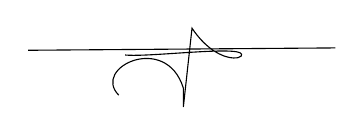
\begin{tikzpicture}[x=1cm,y=1cm]
\draw (0,0.45) -- (3.9,0.48);
\draw (1.15,-0.12) .. controls (0.80,0.23) and (1.75,0.68) .. (1.97,-0.03)
 -- (1.97,-0.27) -- (2.08,0.73)
 .. controls (2.39,0.27) and (2.74,0.33) .. (2.71,0.40)
 .. controls (2.68,0.51) and (1.54,0.36) .. (1.23,0.39);
\end{tikzpicture}}

Filtrations équidimensionnelles et
régulières d'un espace modéré.

Il y en a je présume une qui
est canonique, c'est la \deleted{\unsure{plus}}\inserted{\unsure{moins}} fine
de toutes. [\inserted{\unsure{Plus gén.}} Pour \deleted{\unsure{toute}} filtration
déjà donnée, il y a une filtration
\deleted{plus fine} canonique, régulière
équidimensionnelle, compatible
avec celle-ci] Les invariants de
dévissage de cette filtration sont \unsure{donc}
des invariants de la structure
modérée envisagée.
